\chapter{Testing}

This section is concerned with the testing done on the application. This includes unit tests included within the codebase, performance tests of the API response times and user tests for the client application.

\section{Server tests}

\subsection{Unit tests}

For the server's implementation, we have provided extensive automatic tests using the \texttt{MSTest} framework, which are located in the \texttt{Tests} directory. We have split the tests into 2 namespaces - \texttt{UnitTests} and \texttt{ConnectionSearchTests}. The tests inside \texttt{UnitTests} are intended to check the proper functionality of the individual functions and methods within the code, while the tests inside \texttt{ConnectionSearchTests} test the actual routing functionality as a whole.

In our particular setting, it is close to impossible to test the resulting connections for being the best ones. This is due to the fact that we have many different configuration values and we have no access to an universally correct algorithm that we could compare our results to. Furthermore, due to the large size of processed data, it is not possible to check against manually found best results. Due to all this, the \texttt{ConnectionSearchTests} consist of two types of tests. 

First, we need to check whether all the resulting connections are correct. This includes checking that it departs after (or arrives before) the time specified by the user, that the time between each two consecutive trips is long enough to perform all the transfers and bike trips between them, that no trip taken has invalid stop times or that the starting and ending stops of the result actually correspond to those selected by the user. These tests are present in the \texttt{ResultIntegrityTests}, \texttt{RangeRouteFinderTests} and \texttt{AlternativesRouteFinderTests} classes.

Second, we need to test that the configuration options we provide to our users actually affect what we intend them to affect. Again, apart from a few options (such as forbidding the usage of shared bikes or setting the maximum transfer length), there is no absolute way to whether the result corresponds to the setting values. For this reason, we perform relative testing - for every configuration option, we perform the search for every one of its possible values and compare these results between each other. For example, when testing for the comfort balance requirement (\cref{req:comfort_balance}), we run the search for all 4 values and test that the results with more priority set on speed actually are faster (or at least take the same time) and that the results with more priority set on comfort have less transfers (or at least the same number). These tests can be found in the \texttt{SettingsUsageTests} class.

\subsection{Performance testing}

To test the performance of our application, we have compiled a test file with 1000 combinations of random stop names within the PID public transit network together with random times and byEarlierDeparture settings. To regenerate this file with fresh random values, a Python script is provided in the \texttt{external-testing} directory.

Using Postman's\footnote{https://www.postman.com/} API testing functionality and this file with random stop name pairs, we have performed a request collection of 1000 requests to analyze the program's performance.

\subsubsection{Parameters}

\begin{table}[h!]
\centering
\begin{tabularx}{\textwidth}{|l|X|}
\hline
\textbf{Laptop model} & Lenovo Legion Slim 7 \\
\hline
\textbf{Processor} & AMD Ryzen 7 7840HS \\
\hline
\textbf{Cores (Threads)} & 8 (16) \\
\hline
\textbf{Frequency} & 3.8GHz \\
\hline
\textbf{Memory} & 32GiB DDR5 \\
\hline
\textbf{OS} & Windows 11 Home (23H2) \\
\hline
\end{tabularx}
\caption{Device specification}
\label{tab:device_specification}
\end{table}

\vspace{0.2cm}

% Second table with caption and label
\begin{table}[h!]
\centering
\begin{tabularx}{\textwidth}{|l|X|}
\hline
\textbf{Request count} & 1000 \\
\hline
\textbf{Request interval} & 60 milliseconds \\
\hline
\textbf{Total duration} & 60 seconds \\
\hline
\end{tabularx}
\caption{Test parameters}
\label{tab:test_parameters}
\end{table}

We ran the collection twice - both times, all parameters were randomized except those related to coordinate source or destinations, as there is no impact expected nor observed on those and most of randomly generated points would not be near enough a point within the public transit network. The first run was on a weekday, while the second run was on a weekend to see how the different trip frequency reflects in the results.

The requests were being sent and processed on the same device, meaning internet connection speed has no effect on the results.


\subsubsection{Results}

As you can see in \cref{fig:response_time_histogram}, typically every request takes between 50 and 200 milliseconds to be processed when running the server on the machine we used for testing, with the median time being 124 ms. Considering the use-case of our application, this is a short enough time for the user to not notice any significant delays. The noticeably high number of response times under 20 ms is caused by connection searches for which a connection could not be found due to the source stop not being served by any public transit trips on that day, and thus no further trips and stops needing to be processed.

As is visible in \cref{fig:success_rates}, the number of connections that could not be found is significantly higher during the weekend. This is caused by many of the randomly selected stops being located in small villages or similar places, where there may be no service at all on weekends and where they might be too far from any served stop to be reached by a (short enough) transfer. As the vast majority of population within the Central Bohemian region served by PID lives directly in Prague and in the surrounding major cities, connections to these sparsely populated rural stops that are not served on weekends are much less likely to be searched for and thus this is not a major issue.

As expected, the response times are slightly longer when the search is performed on a weekday. Presumably, this is due to having to process the higher number of trips operating on weekdays as opposed to weekends. However, the difference is only small. The response time is more significantly impacted by other factors, especially the density of the network around the source point and the distance between the two points. This is due to the nature of the RAPTOR algorithm we have used (for more details, see \cref{subsec:public_transit_routing} and \textcite{delling2015raptor}).

\begin{figure}[h!]
    \centering
    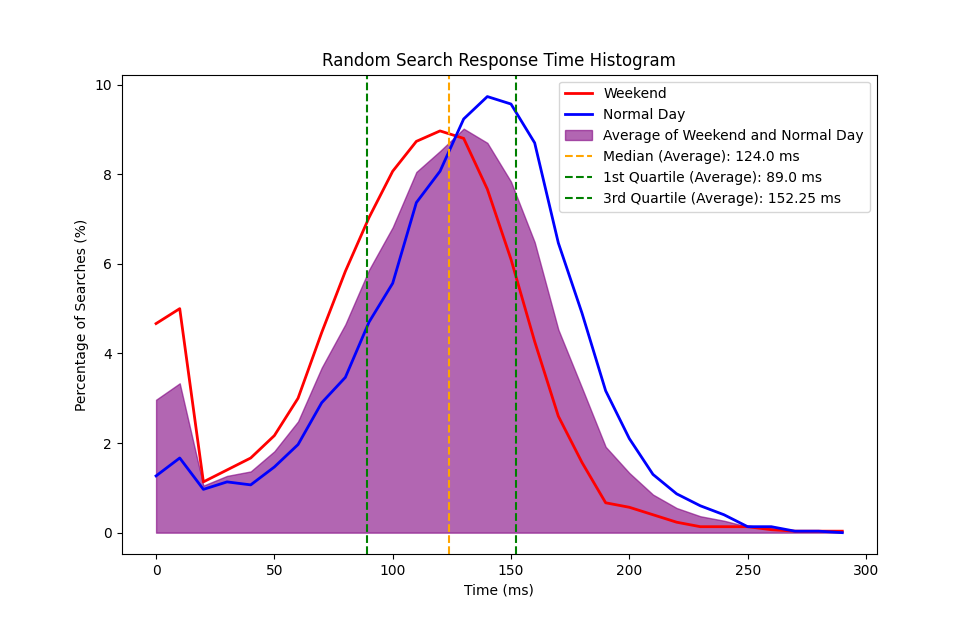
\includegraphics[width=\textwidth]{img/histogram.png}
    \caption{Histogram of response times}
    \label{fig:response_time_histogram}
\end{figure}

\begin{figure}[h!]
    \centering
    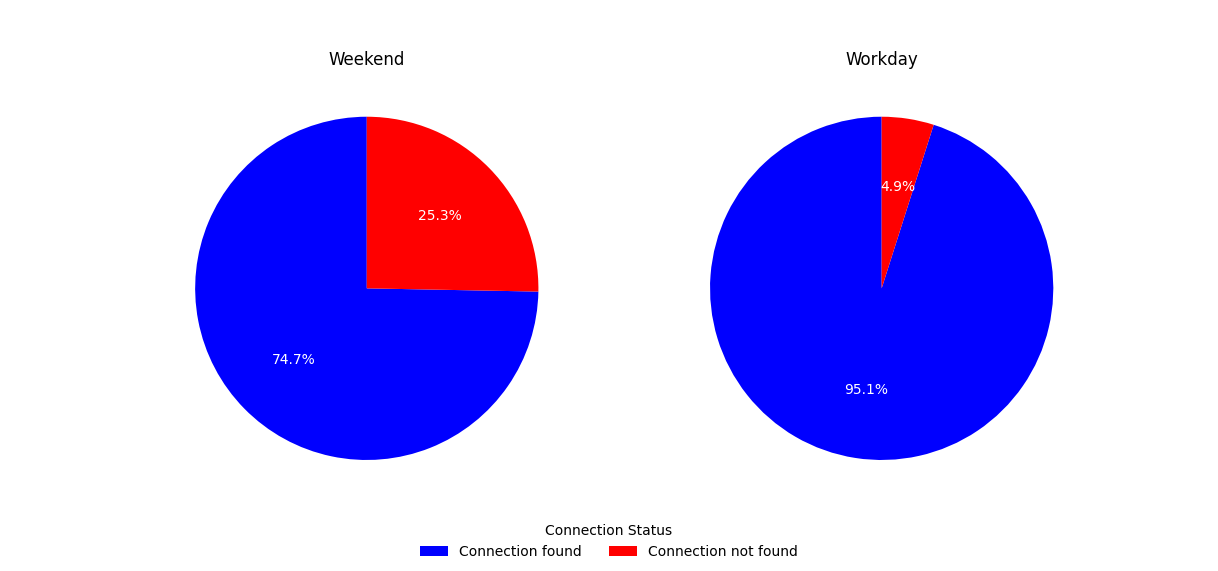
\includegraphics[width=\textwidth]{img/success_rates.png}
    \caption{Found connections rates}
    \label{fig:success_rates}
\end{figure}


\section{Client tests}

\subsection{User testing}

To properly test our client application and ensure that all functional requirements we set out to fulfill are met, we have prepared a list of test cases to perform manual user testing of the client. These contain the steps that the tester should perform and the expected results that these steps should lead to. We have performed all of these tests to ensure our application is working correctly. All the test cases can be found in the client repository.

\subsection{Usability testing}

\xxx{Results of questionnaire for alpha users}